\subsection{Early Returning Agreement}

\pgfdeclarelayer{background}
\pgfdeclarelayer{foreground}
\pgfsetlayers{background,main,foreground}

\newcommand{\pie}[1]{%
\begin{tikzpicture}
 \draw (0,0) circle (.3em);\fill (.3em,0) arc (0:#1:.3em) -- (0,0) -- cycle;
\end{tikzpicture}%
}

\def\stateUP{\textcolor{black}{\ensuremath{\uparrow}}}
\def\stateDOWN{\textcolor{black}{\ensuremath{\downarrow}}}
\def\stateNOTPART{\textcolor{black}{\ensuremath{?}}}
\def\stateDECIDED{\textcolor{black}{\ensuremath{\pie{360}}}}

\def\msgPART{\textcolor{blue!75}{\ensuremath{\pie{180}}}}
\def\msgDECIDE{\textcolor{blue!75}{\ensuremath{\pie{360}}}}
\def\msgRR{\textcolor{blue!75}{\textbf{?}}}

\renewcommand{\proc}[2]{\expandafter\gdef\csname proc:#1:style\endcsname{alivenode}
\ifcase#2
% Case 0
\expandafter\gdef\csname proc:#1:label\endcsname{\stateUP}
\or
% Case 1
\expandafter\gdef\csname proc:#1:label\endcsname{\stateDOWN}
\or
% Case 2
\expandafter\gdef\csname proc:#1:label\endcsname{\stateNOTPART}
\or
% Case 3
\expandafter\gdef\csname proc:#1:label\endcsname{\ensuremath{#1}}
\or
% Case 4
\expandafter\gdef\csname proc:#1:label\endcsname{\stateDECIDED}
\or
%Case 5
\expandafter\gdef\csname proc:#1:label\endcsname{}
\expandafter\gdef\csname proc:#1:style\endcsname{deadnode}
\fi}
\newcommand{\state}[1]{\foreach \x [count=\xi] in {#1} {\proc{\xi}{\x}}}
\newcommand{\proclabel}[1]{\csname proc:#1:label\endcsname\relax}
\newcommand{\procstyle}[1]{\csname proc:#1:style\endcsname\relax}
\tikzstyle{alivenode} = [draw,shape=circle,minimum size=.75cm,inner sep=0pt,fill=blue!20]
\tikzstyle{deadnode} = [draw,shape=circle,minimum size=.75cm,inner sep=0pt,fill=blue!5,text=blue!5,draw=black!10]
\tikzstyle{aliveedge} = [draw=black,line width=1]
\tikzstyle{deadedge} = [draw=black!10,line width=1]
\newcommand{\msgtype}[1]{\ifcase#1
% Case 0
\ensuremath{\msgPART}
\or
% Case 1
\ensuremath{\msgDECIDE}
\or
% Case 2
\msgRR
\fi}
\def\msg#1#2#3{\path[->] (P#1) edge[blue!75,bend right=30,pos=.5] node[draw=blue!75,fill=white,inner sep=2pt,scale=0.5] {\msgtype{#3}} (P#2);}
\def\monitor#1#2{\pgfmathanglebetweenpoints{\pgfpointanchor{P#1}{center}}{\pgfpointanchor{P#2}{center}}%
\pgfmathsetmacro{\angle}{\pgfmathresult - 90}%
\path[] (P#1) edge[near start] node[rotate=\angle] {
\includegraphics[width=.35cm]{FD.png}} (P#2);}
\def\monitoring{
\includegraphics[width=.35cm,angle=270,origin=c]{FD.png}}


\begin{frame}
  \frametitle{Consensus in the context of HPC}

  Consider the case of a broadcast implemented with a binary tree.

      \resizebox{\linewidth}{!}{\begin{tikzpicture}[>=latex',scale=.25]
          \node[draw,alivenode] (root) at (0, 0) {\textcolor{green}{\checked}};
          \node[draw,deadnode] (L) at (-10, -3) {};
          \node[draw,alivenode] (R) at (10, -3) {\textcolor{green}{\checked}};
          \node[draw,alivenode] (LL) at (-15, -6) {\textcolor{red}{$\times$}};
          \node[draw,alivenode] (LR) at (-5, -6) {\textcolor{red}{$\times$}};
          \node[draw,alivenode] (RL) at (5, -6) {\textcolor{green}{\checked}};
          \node[draw,alivenode] (RR) at (15, -6){\textcolor{green}{\checked}};
          \draw (root) edge[->,dashed] (L);
          \draw (root) edge[->] (R);
          \draw (L) edge[->,dashed] (LL);
          \draw (L) edge[->,dashed] (LR);
          \draw (R) edge[->] (RL);
          \draw (R) edge[->] (RR);
        \end{tikzpicture}}

      Failures, that happen during the execution, introduce
      inconsistencies: not all processes know that the broadcast
      operation failed.

      \begin{center}
      Consensus (or agreement) allows to reconcile inconsistent /
      non-uniform states \textcolor{red}{due to failures}.

      It must be \textcolor{green!65!black}{reliable}.

      It must be \textcolor{green!65!black}{efficient}, especially in
      the \textcolor{green!65!black}{failure-free} case.
      \end{center}

\end{frame}

\begin{comment}
\begin{frame}[t]
  \frametitle{ULFM Agreement Specification}

  \texttt{int MPIX\_Comm\_agree(MPI\_Comm comm, int *flag);}\\
  \texttt{MPIX\_COMM\_AGREE(COMM, FLAG, IERROR)}\\
  ~\qquad\qquad\texttt{  INTEGER COMM, FLAG, IERROR}

  \begin{description}
  \item[\texttt{comm}] the communicator on which to apply the
    consensus
  \item[\texttt{flag}] An in/out integer: in input, the process
    participation, in output, the result of the agreement on these
    ints (bitwise and)
  \item[\texttt{return value}] An error code if new process failures
    were discovered during the agreement, or success
  \end{description}
  
  The operation implements an agreement on the couple
  \texttt{(flag, return code)}: all surviving process, despite any 
  failure have the same values in each (even if the return code is an
  error, flag is defined).
 
\end{frame}
\end{comment}

\begin{frame}
  \frametitle{Specification}

  \begin{beamerboxesrounded}{Correctness}
    \begin{description}
    \item[Termination] Every living process eventually decides.
    \item[Integrity] Once a living process decides a value, it remains decided on that value.
    \item[Agreement] No two living processes decide differently.
    \item[Participation] When a process decides upon a value, it
      contributed to the decided value.
    \end{description}
  \end{beamerboxesrounded}

\bigskip

  Traditional consensus relies on \textcolor{green!75!black}{Validity}\\
  This is because \textcolor{red}{one} value is \textcolor{red}{chosen}.

\end{frame}

\begin{frame}
  \frametitle{Assumptions}
  
  \begin{itemize}
  \item Processes have totally ordered, \textcolor{red!75}{unique identifiers}
  \item Any process belonging to a group knows
    \textcolor{blue!75}{what processes belong to that group}
  \item Any process may be subject to a \textcolor{red!75}{permanent failure}
  \item The network does not \textcolor{blue!50!black}{lose},
    \textcolor{red!50!black}{modify}, nor
    \textcolor{green!50!black}{duplicate} messages, but communication
    delays \textcolor{red!75}{have \emph{unknown} bounds}
  \item The system provides a \textcolor{red!50!black}{Perfect Failure
      Detector} (${\mathcal P}$):
    \begin{itemize}
    \item All \textcolor{red!50!black}{incorrect} processes are eventually suspected by all
      \textcolor{green!50!black}{correct} processes
    \item No \textcolor{green!50!black}{correct} process is ever suspected by any process
    \end{itemize}
  \item The operation of the consensus is associative and commutative,
    and idempotent, with a \emph{known neutral element}
  \end{itemize}

\end{frame}


\begin{frame}
  \frametitle{\only<1>{Principle}\only<2>{Notation}}
  \begin{columns}[T] % align columns
    \begin{column}{.30\textwidth}
      \begin{center}
      \resizebox{.8\linewidth}{!}{\begin{tikzpicture}[>=latex',scale=.25]
          \node (n) at (0,0) [alivenode] {$$};
          \node (p) at (0,6) {parent};
          \node (lc) at (-6,-6) {left child};
          \node (rc) at (6,-6) {right child};
          \draw (n) edge [aliveedge] (p);
          \draw (n) edge [aliveedge] (lc);
          \draw (n) edge [aliveedge] (rc);
        \end{tikzpicture}}

      \resizebox{.8\linewidth}{!}{\begin{tikzpicture}[>=latex',scale=.25]
          \node (Pn) at (0,0) [alivenode] {\stateUP};
          \node (Pp) at (0,6)  [alivenode] {\stateDOWN};
          \node (Plc) at (-6,-6)  [alivenode] {\stateNOTPART};
          \node (Prc) at (6,-6)  [alivenode] {\stateDECIDED};
          \draw (Pn) edge [aliveedge] (Pp);
          \draw (Pn) edge [aliveedge] (Plc);
          \draw (Pn) edge [aliveedge] (Prc);
          \msg{n}{p}{0}
          \msg{n}{lc}{1}
          \msg{n}{rc}{2}
          \monitor{n}{p}
          \monitor{n}{rc}\monitor{rc}{n}
      \end{tikzpicture}}
      \end{center}
    \end{column}%
    \hfill%
    \begin{column}{.75\textwidth}
\only<1>{
    \begin{itemize}
    \item Processes are arranged following a \textcolor{red}{mendable tree} topology:
      given a list of known dead processes, they communicate or monitor
      the liveliness of only their neighbors in that topology. 
    \item The algorithm is a \textcolor{blue}{resilient version} of Fan-in / Fan-out: all
      contributions (noted \msgPART) are reduced along the tree up to
      the root, that broadcasts it
    \item \emph{Deciding} the result of the consensus for a given
      process consists in \textcolor{red}{remembering} the return value of the
      consensus, \textcolor{blue}{broadcasting} it to the current children, and
      \textcolor{red}{returning} \textit{as if} the consensus was completed.
    \end{itemize}}
\only<2>{
  \footnotesize
  \begin{itemize}
  \item Alive processes can be in 3 states:
    \begin{itemize}
    \item \stateNOTPART, if they have not entered the consensus yet
    \item \stateUP, if they are waiting from the contribution of their
      children
    \item \stateDOWN, if they have sent their contribution to their
      parent and are waiting for the decision
    \item \stateDECIDED, if they have received the decision
    \end{itemize}
  \item There are 3 types of messages:
    \begin{itemize}
    \item \msgPART, when a process sends its participation to a parent
    \item \msgDECIDE, when a process broadcasts the decision to its
      children
    \item \msgRR, when a process enquired about a possible result of
      a completed consensus
    \end{itemize}
  \item Processes can monitor (\monitoring) other processes for failures
  \end{itemize}
}
  \end{column}
  \end{columns}
\end{frame}

\begin{frame}[fragile]
  \frametitle{Mendable Tree for Consensus}

\begin{center}
\resizebox{.45\linewidth}{!}{\begin{tikzpicture}[>=latex',scale=.25]
\proc{1}{3}\proc{2}{3}\proc{3}{3}\proc{4}{3}\proc{5}{3}
\proc{6}{3}\proc{7}{3}\proc{8}{3}\proc{9}{3}\proc{10}{3}
\proc{11}{3}\proc{12}{3}\proc{13}{3}\proc{14}{3}\proc{15}{3}
%%
\node (P2) at (336.0bp,252.5bp) [\procstyle{2}] {$\proclabel{2}$};
  \node (P3) at (494.0bp,252.5bp) [\procstyle{3}] {$\proclabel{3}$};
  \node (P1) at (408.0bp,375.5bp) [\procstyle{1}] {$\proclabel{1}$};
  \node (P6) at (494.0bp,129.5bp) [\procstyle{6}] {$\proclabel{6}$};
  \node (P7) at (666.0bp,129.5bp) [\procstyle{7}] {$\proclabel{7}$};
  \node (P4) at (116.0bp,129.5bp) [\procstyle{4}] {$\proclabel{4}$};
  \node (P5) at (336.0bp,129.5bp) [\procstyle{5}] {$\proclabel{5}$};
  \node (P8) at (6.0bp,6.5bp) [\procstyle{8}] {$\proclabel{8}$};
  \node (P9) at (116.0bp,6.5bp) [\procstyle{9}] {$\proclabel{9}$};
  \node (P10) at (226.0bp,6.5bp) [\procstyle{10}] {$\proclabel{10}$};
  \node (P11) at (336.0bp,6.5bp) [\procstyle{11}] {$\proclabel{11}$};
  \node (P12) at (446.0bp,6.5bp) [\procstyle{12}] {$\proclabel{12}$};
  \node (P13) at (556.0bp,6.5bp) [\procstyle{13}] {$\proclabel{13}$};
  \node (P14) at (666.0bp,6.5bp) [\procstyle{14}] {$\proclabel{14}$};
  \node (P15) at (776.0bp,6.5bp) [\procstyle{15}] {$\proclabel{15}$};
%
  \draw [aliveedge] (P4) -- node {$$} (P9);
  \draw [aliveedge] (P4) -- node {$$} (P8);
  \draw [aliveedge] (P6) -- node {$$} (P13);
  \draw [aliveedge] (P3) -- node {$$} (P7);
  \draw [aliveedge] (P1) -- node {$$} (P2);
  \draw [aliveedge] (P6) -- node {$$} (P12);
  \draw [aliveedge] (P1) -- node {$$} (P3);
  \draw [aliveedge] (P3) -- node {$$} (P6);
  \draw [aliveedge] (P2) -- node {$$} (P4);
  \draw [aliveedge] (P7) -- node {$$} (P14);
  \draw [aliveedge] (P5) -- node {$$} (P10);
  \draw [aliveedge] (P2) -- node {$$} (P5);
  \draw [aliveedge] (P5) -- node {$$} (P11);
  \draw [aliveedge] (P7) -- node {$$} (P15);
\end{tikzpicture}}
\hspace{\stretch{1}}
\only<1>{\resizebox{.45\linewidth}{!}{\begin{tikzpicture}[>=latex',scale=.25]
\proc{1}{3}\proc{2}{3}\proc{3}{5}\proc{4}{3}\proc{5}{3}
\proc{6}{5}\proc{7}{3}\proc{8}{3}\proc{9}{3}\proc{10}{3}
\proc{11}{3}\proc{12}{3}\proc{13}{5}\proc{14}{3}\proc{15}{3}
%%
\node (P2) at (336.0bp,252.5bp) [\procstyle{2}] {$\proclabel{2}$};
  \node (P3) at (494.0bp,252.5bp) [\procstyle{3}] {$\proclabel{3}$};
  \node (P1) at (408.0bp,375.5bp) [\procstyle{1}] {$\proclabel{1}$};
  \node (P6) at (494.0bp,129.5bp) [\procstyle{6}] {$\proclabel{6}$};
  \node (P7) at (666.0bp,129.5bp) [\procstyle{7}] {$\proclabel{7}$};
  \node (P4) at (116.0bp,129.5bp) [\procstyle{4}] {$\proclabel{4}$};
  \node (P5) at (336.0bp,129.5bp) [\procstyle{5}] {$\proclabel{5}$};
  \node (P8) at (6.0bp,6.5bp) [\procstyle{8}] {$\proclabel{8}$};
  \node (P9) at (116.0bp,6.5bp) [\procstyle{9}] {$\proclabel{9}$};
  \node (P10) at (226.0bp,6.5bp) [\procstyle{10}] {$\proclabel{10}$};
  \node (P11) at (336.0bp,6.5bp) [\procstyle{11}] {$\proclabel{11}$};
  \node (P12) at (446.0bp,6.5bp) [\procstyle{12}] {$\proclabel{12}$};
  \node (P13) at (556.0bp,6.5bp) [\procstyle{13}] {$\proclabel{13}$};
  \node (P14) at (666.0bp,6.5bp) [\procstyle{14}] {$\proclabel{14}$};
  \node (P15) at (776.0bp,6.5bp) [\procstyle{15}] {$\proclabel{15}$};
%
  \draw [aliveedge] (P1) -- node {$$} (P2);
  % \draw [aliveedge] (P1) -- node {$$} (P3);
  \draw [aliveedge] (P2) -- node {$$} (P4);
  \draw [aliveedge] (P2) -- node {$$} (P5);
  % \draw [aliveedge] (P3) -- node {$$} (P7);
  % \draw [aliveedge] (P3) -- node {$$} (P6);
  \draw [aliveedge] (P4) -- node {$$} (P8);
  \draw [aliveedge] (P4) -- node {$$} (P9);
  \draw [aliveedge] (P5) -- node {$$} (P10);
  \draw [aliveedge] (P5) -- node {$$} (P11);
  % \draw [aliveedge] (P6) -- node {$$} (P13);
  % \draw [aliveedge] (P6) -- node {$$} (P12);
  \draw [aliveedge] (P7) -- node {$$} (P14);
  \draw [aliveedge] (P7) -- node {$$} (P15);
  \draw [aliveedge] (P12) -- node {$$} (P1);
  \draw [aliveedge] (P7) -- node {$$} (P1);
\end{tikzpicture}}}
\only<2>{\resizebox{.45\linewidth}{!}{\begin{tikzpicture}[>=latex',scale=.25]
\proc{1}{5}\proc{2}{5}\proc{3}{3}\proc{4}{3}\proc{5}{3}
\proc{6}{3}\proc{7}{3}\proc{8}{3}\proc{9}{3}\proc{10}{3}
\proc{11}{3}\proc{12}{3}\proc{13}{3}\proc{14}{3}\proc{15}{3}
%%
\node (P2) at (336.0bp,252.5bp) [\procstyle{2}] {$\proclabel{2}$};
  \node (P3) at (494.0bp,252.5bp) [\procstyle{3}] {$\proclabel{3}$};
  \node (P1) at (408.0bp,375.5bp) [\procstyle{1}] {$\proclabel{1}$};
  \node (P6) at (494.0bp,129.5bp) [\procstyle{6}] {$\proclabel{6}$};
  \node (P7) at (666.0bp,129.5bp) [\procstyle{7}] {$\proclabel{7}$};
  \node (P4) at (116.0bp,129.5bp) [\procstyle{4}] {$\proclabel{4}$};
  \node (P5) at (336.0bp,129.5bp) [\procstyle{5}] {$\proclabel{5}$};
  \node (P8) at (6.0bp,6.5bp) [\procstyle{8}] {$\proclabel{8}$};
  \node (P9) at (116.0bp,6.5bp) [\procstyle{9}] {$\proclabel{9}$};
  \node (P10) at (226.0bp,6.5bp) [\procstyle{10}] {$\proclabel{10}$};
  \node (P11) at (336.0bp,6.5bp) [\procstyle{11}] {$\proclabel{11}$};
  \node (P12) at (446.0bp,6.5bp) [\procstyle{12}] {$\proclabel{12}$};
  \node (P13) at (556.0bp,6.5bp) [\procstyle{13}] {$\proclabel{13}$};
  \node (P14) at (666.0bp,6.5bp) [\procstyle{14}] {$\proclabel{14}$};
  \node (P15) at (776.0bp,6.5bp) [\procstyle{15}] {$\proclabel{15}$};
%
%  \draw [aliveedge] (P1) -- node {$$} (P2);
%  \draw [aliveedge] (P1) -- node {$$} (P3);
%  \draw [aliveedge] (P2) -- node {$$} (P4);
%  \draw [aliveedge] (P2) -- node {$$} (P5);
  \draw [aliveedge] (P3) -- node {$$} (P4);
  \draw [aliveedge] (P3) -- node {$$} (P5);
  \draw [aliveedge] (P3) -- node {$$} (P7);
  \draw [aliveedge] (P3) -- node {$$} (P6);
  \draw [aliveedge] (P4) -- node {$$} (P8);
  \draw [aliveedge] (P4) -- node {$$} (P9);
  \draw [aliveedge] (P5) -- node {$$} (P10);
  \draw [aliveedge] (P5) -- node {$$} (P11);
  \draw [aliveedge] (P6) -- node {$$} (P13);
  \draw [aliveedge] (P6) -- node {$$} (P12);
  \draw [aliveedge] (P7) -- node {$$} (P14);
  \draw [aliveedge] (P7) -- node {$$} (P15);
\end{tikzpicture}}}
\only<3>{\resizebox{.45\linewidth}{!}{\begin{tikzpicture}[>=latex',scale=.25]
\proc{1}{5}\proc{2}{5}\proc{3}{5}\proc{4}{5}\proc{5}{5}
\proc{6}{5}\proc{7}{5}\proc{8}{3}\proc{9}{3}\proc{10}{3}
\proc{11}{3}\proc{12}{3}\proc{13}{3}\proc{14}{3}\proc{15}{3}
%%
\node (P2) at (336.0bp,252.5bp) [\procstyle{2}] {$\proclabel{2}$};
  \node (P3) at (494.0bp,252.5bp) [\procstyle{3}] {$\proclabel{3}$};
  \node (P1) at (408.0bp,375.5bp) [\procstyle{1}] {$\proclabel{1}$};
  \node (P6) at (494.0bp,129.5bp) [\procstyle{6}] {$\proclabel{6}$};
  \node (P7) at (666.0bp,129.5bp) [\procstyle{7}] {$\proclabel{7}$};
  \node (P4) at (116.0bp,129.5bp) [\procstyle{4}] {$\proclabel{4}$};
  \node (P5) at (336.0bp,129.5bp) [\procstyle{5}] {$\proclabel{5}$};
  \node (P8) at (6.0bp,6.5bp) [\procstyle{8}] {$\proclabel{8}$};
  \node (P9) at (116.0bp,6.5bp) [\procstyle{9}] {$\proclabel{9}$};
  \node (P10) at (226.0bp,6.5bp) [\procstyle{10}] {$\proclabel{10}$};
  \node (P11) at (336.0bp,6.5bp) [\procstyle{11}] {$\proclabel{11}$};
  \node (P12) at (446.0bp,6.5bp) [\procstyle{12}] {$\proclabel{12}$};
  \node (P13) at (556.0bp,6.5bp) [\procstyle{13}] {$\proclabel{13}$};
  \node (P14) at (666.0bp,6.5bp) [\procstyle{14}] {$\proclabel{14}$};
  \node (P15) at (776.0bp,6.5bp) [\procstyle{15}] {$\proclabel{15}$};
%
  \draw [aliveedge] (P8) edge[bend left=10] node {$$} (P9);
  \draw [aliveedge] (P8) edge[bend right=10] node {$$} (P10);
  \draw [aliveedge] (P8) edge[bend left=15] node {$$} (P11);
  \draw [aliveedge] (P8) edge[bend right=15] node {$$} (P12);
  \draw [aliveedge] (P8) edge[bend left=20] node {$$} (P13);
  \draw [aliveedge] (P8) edge[bend right=20] node {$$} (P14);
  \draw [aliveedge] (P8) edge[bend left=25] node {$$} (P15);
\end{tikzpicture}}}
\end{center}

\only<1>{ The Fan-in Fan-out tree used during the consensus is
  \textcolor{green!75}{mended}, as failures are discovered during the
  execution.

  The mending rule is simple: processes are arranged according to
  their (MPI) rank following a \textcolor{red!75}{breath-first} search
  of the tree}

\only<2>{ Nodes replace their parents by the
  \textcolor{red!75}{highest-ranked alive ancester} in the tree in
  case of failure.
  
  Processes without an alive ancestor in the original tree connect to
  the \textcolor{red!75}{lowest alive processor} as their
  parent. \emph{The lowest alive processor is always the root of the
    tree} }

\only<3>{If half the processes die, the tree can, in the worst case,
  degenerate to a \textcolor{blue!75}{$np/2$-degree star}}

\end{frame}

\begin{frame}[fragile]
  \frametitle{Architecture-Aware Tree}

  \begin{center}
    \resizebox{\linewidth}{!}{\begin{tikzpicture}[>=latex',scale=.25]
          \node (P3_9) at (1619.0bp,164.0bp) [alivenode] {$$};
  \node (P1_a) at (1015.0bp,310.0bp) [alivenode] {$$};
  \node (P3_8) at (1509.0bp,164.0bp) [alivenode] {$$};
  \node (P1_0) at (1086.0bp,748.0bp) [alivenode] {$$};
  \node (P1_1) at (1017.0bp,602.0bp) [alivenode] {$$};
  \node (P1_2) at (1154.0bp,602.0bp) [alivenode] {$$};
  \node (P1_3) at (905.0bp,456.0bp) [alivenode] {$$};
  \node (P1_4) at (1015.0bp,456.0bp) [alivenode] {$$};
  \node (P1_5) at (1154.0bp,456.0bp) [alivenode] {$$};
  \node (P1_6) at (1345.0bp,456.0bp) [alivenode] {$$};
  \node (P1_7) at (685.0bp,310.0bp) [alivenode] {$$};
  \node (P0_1) at (302.0bp,748.0bp) [alivenode] {$$};
  \node (P1_9) at (905.0bp,310.0bp) [alivenode] {$$};
  \node (P0_3) at (137.0bp,602.0bp) [alivenode] {$$};
  \node (P0_2) at (769.0bp,748.0bp) [alivenode] {$$};
  \node (P0_5) at (577.0bp,602.0bp) [alivenode] {$$};
  \node (P0_4) at (302.0bp,602.0bp) [alivenode] {$$};
  \node (P0_7) at (27.0bp,456.0bp) [alivenode] {$$};
  \node (P0_6) at (769.0bp,602.0bp) [alivenode] {$$};
  \node (P3_6) at (2059.0bp,310.0bp) [alivenode] {$$};
  \node (P3_7) at (1399.0bp,164.0bp) [alivenode] {$$};
  \node (P3_4) at (1675.0bp,310.0bp) [alivenode] {$$};
  \node (P3_5) at (1892.0bp,310.0bp) [alivenode] {$$};
  \node (P3_2) at (1892.0bp,456.0bp) [alivenode] {$$};
  \node (P3_3) at (1563.0bp,310.0bp) [alivenode] {$$};
  \node (P3_0) at (1620.0bp,602.0bp) [alivenode] {$$};
  \node (P3_1) at (1620.0bp,456.0bp) [alivenode] {$$};
  \node (P2_7) at (2223.0bp,310.0bp) [alivenode] {$$};
  \node (P2_6) at (2882.0bp,456.0bp) [alivenode] {$$};
  \node (P2_5) at (2717.0bp,456.0bp) [alivenode] {$$};
  \node (P2_4) at (2442.0bp,456.0bp) [alivenode] {$$};
  \node (P2_3) at (2332.0bp,456.0bp) [alivenode] {$$};
  \node (P2_2) at (2717.0bp,602.0bp) [alivenode] {$$};
  \node (P2_1) at (2387.0bp,602.0bp) [alivenode] {$$};
  \node (P2_0) at (2387.0bp,748.0bp) [alivenode] {$$};
  \node (P0_9) at (247.0bp,456.0bp) [alivenode] {$$};
  \node (P2_9) at (2442.0bp,310.0bp) [alivenode] {$$};
  \node (P0_8) at (137.0bp,456.0bp) [alivenode] {$$};
  \node (P2_8) at (2332.0bp,310.0bp) [alivenode] {$$};
  \node (P3_f) at (1399.0bp,18.0bp) [alivenode] {$$};
  \node (P3_d) at (2059.0bp,164.0bp) [alivenode] {$$};
  \node (P3_e) at (2169.0bp,164.0bp) [alivenode] {$$};
  \node (P3_b) at (1839.0bp,164.0bp) [alivenode] {$$};
  \node (P3_c) at (1949.0bp,164.0bp) [alivenode] {$$};
  \node (P3_a) at (1729.0bp,164.0bp) [alivenode] {$$};
  \node (P2_f) at (2279.0bp,164.0bp) [alivenode] {$$};
  \node (P2_e) at (2992.0bp,310.0bp) [alivenode] {$$};
  \node (P2_d) at (2882.0bp,310.0bp) [alivenode] {$$};
  \node (P2_c) at (2772.0bp,310.0bp) [alivenode] {$$};
  \node (P2_b) at (2662.0bp,310.0bp) [alivenode] {$$};
  \node (P2_a) at (2552.0bp,310.0bp) [alivenode] {$$};
  \node (P1_8) at (795.0bp,310.0bp) [alivenode] {$$};
  \node (P1_b) at (1125.0bp,310.0bp) [alivenode] {$$};
  \node (P1_c) at (1235.0bp,310.0bp) [alivenode] {$$};
  \node (P1_d) at (1345.0bp,310.0bp) [alivenode] {$$};
  \node (P1_e) at (1455.0bp,310.0bp) [alivenode] {$$};
  \node (P1_f) at (685.0bp,164.0bp) [alivenode] {$$};
  \node (P0_0) at (879.0bp,894.0bp) [alivenode] {$$};
  \node (P0_a) at (357.0bp,456.0bp) [alivenode] {$$};
  \node (P0_c) at (577.0bp,456.0bp) [alivenode] {$$};
  \node (P0_b) at (467.0bp,456.0bp) [alivenode] {$$};
  \node (P0_e) at (797.0bp,456.0bp) [alivenode] {$$};
  \node (P0_d) at (687.0bp,456.0bp) [alivenode] {$$};
  \node (P0_f) at (27.0bp,310.0bp) [alivenode] {$$};
  \draw [aliveedge] (P1_0) -- node {$$} (P3_0);
  \draw [aliveedge] (P1_2) -- node {$$} (P1_6);
  \draw [aliveedge] (P0_1) -- node {$$} (P0_4);
  \draw [aliveedge] (P3_2) -- node {$$} (P3_5);
  \draw [aliveedge] (P0_4) -- node {$$} (P0_a);
  \draw [aliveedge] (P0_0) -- node {$$} (P0_1);
  \draw [aliveedge] (P3_6) -- node {$$} (P3_d);
  \draw [aliveedge] (P1_1) -- node {$$} (P1_4);
  \draw [aliveedge] (P1_5) -- node {$$} (P1_c);
  \draw [aliveedge] (P3_1) -- node {$$} (P3_3);
  \draw [aliveedge] (P2_0) -- node {$$} (P2_2);
  \draw [aliveedge] (P2_2) -- node {$$} (P2_6);
  \draw [aliveedge] (P1_7) -- node {$$} (P1_f);
  \draw [aliveedge] (P2_4) -- node {$$} (P2_9);
  \draw [aliveedge] (P2_3) -- node {$$} (P2_7);
  \draw [aliveedge] (P1_0) -- node {$$} (P1_1);
  \draw [aliveedge] (P3_0) -- node {$$} (P3_2);
  \draw [aliveedge] (P0_0) -- node {$$} (P1_0);
  \draw [aliveedge] (P3_0) -- node {$$} (P3_1);
  \draw [aliveedge] (P0_7) -- node {$$} (P0_f);
  \draw [aliveedge] (P3_4) -- node {$$} (P3_a);
  \draw [aliveedge] (P2_4) -- node {$$} (P2_a);
  \draw [aliveedge] (P2_1) -- node {$$} (P2_3);
  \draw [aliveedge] (P0_5) -- node {$$} (P0_c);
  \draw [aliveedge] (P3_6) -- node {$$} (P3_e);
  \draw [aliveedge] (P1_5) -- node {$$} (P1_b);
  \draw [aliveedge] (P0_1) -- node {$$} (P0_3);
  \draw [aliveedge] (P3_5) -- node {$$} (P3_c);
  \draw [aliveedge] (P1_3) -- node {$$} (P1_8);
  \draw [aliveedge] (P0_0) -- node {$$} (P0_2);
  \draw [aliveedge] (P2_0) -- node {$$} (P2_1);
  \draw [aliveedge] (P1_0) -- node {$$} (P1_2);
  \draw [aliveedge] (P2_6) -- node {$$} (P2_e);
  \draw [aliveedge] (P1_1) -- node {$$} (P1_3);
  \draw [aliveedge] (P0_5) -- node {$$} (P0_b);
  \draw [aliveedge] (P3_5) -- node {$$} (P3_b);
  \draw [aliveedge] (P2_6) -- node {$$} (P2_d);
  \draw [aliveedge] (P3_3) -- node {$$} (P3_7);
  \draw [aliveedge] (P3_3) -- node {$$} (P3_8);
  \draw [aliveedge] (P0_6) -- node {$$} (P0_d);
  \draw [aliveedge] (P1_6) -- node {$$} (P1_e);
  \draw [aliveedge] (P0_3) -- node {$$} (P0_8);
  \draw [aliveedge] (P0_0) -- node {$$} (P2_0);
  \draw [aliveedge] (P2_5) -- node {$$} (P2_c);
  \draw [aliveedge] (P1_3) -- node {$$} (P1_7);
  \draw [aliveedge] (P1_2) -- node {$$} (P1_5);
  \draw [aliveedge] (P2_7) -- node {$$} (P2_f);
  \draw [aliveedge] (P0_2) -- node {$$} (P0_5);
  \draw [aliveedge] (P2_1) -- node {$$} (P2_4);
  \draw [aliveedge] (P1_4) -- node {$$} (P1_9);
  \draw [aliveedge] (P2_3) -- node {$$} (P2_8);
  \draw [aliveedge] (P1_4) -- node {$$} (P1_a);
  \draw [aliveedge] (P2_5) -- node {$$} (P2_b);
  \draw [aliveedge] (P0_6) -- node {$$} (P0_e);
  \draw [aliveedge] (P1_6) -- node {$$} (P1_d);
  \draw [aliveedge] (P0_3) -- node {$$} (P0_7);
  \draw [aliveedge] (P3_1) -- node {$$} (P3_4);
  \draw [aliveedge] (P3_4) -- node {$$} (P3_9);
  \draw [aliveedge] (P0_2) -- node {$$} (P0_6);
  \draw [aliveedge] (P2_2) -- node {$$} (P2_5);
  \draw [aliveedge] (P3_7) -- node {$$} (P3_f);
  \draw [aliveedge] (P0_4) -- node {$$} (P0_9);
  \draw [aliveedge] (P3_2) -- node {$$} (P3_6);
        \begin{pgfonlayer}{background}
%node 0
          \draw[rounded corners=2em,line width=3em,red!20,cap=round]
          (P0_0.center) -- (P0_1.center) -- (P0_3.center) -- (P0_7.center)  -- (P0_f.center);
          \draw[rounded corners=2em,line width=3em,red!20,cap=round]
          (P0_0.center) -- (P0_2.center) -- (P0_5.center) --
          (P0_b.center);
          \draw[rounded corners=2em,line width=3em,red!20,cap=round]
          (P0_1.center) -- (P0_4.center) -- (P0_9.center);
          \draw[rounded corners=2em,line width=3em,red!20,cap=round]
          (P0_4.center) -- (P0_a.center);
          \draw[rounded corners=2em,line width=3em,red!20,cap=round]
          (P0_2.center) -- (P0_5.center) -- (P0_b.center);
          \draw[rounded corners=2em,line width=3em,red!20,cap=round]
          (P0_5.center) -- (P0_c.center);
          \draw[rounded corners=2em,line width=3em,red!20,cap=round]
          (P0_2.center) -- (P0_6.center) -- (P0_d.center);
          \draw[rounded corners=2em,line width=3em,red!20,cap=round]
          (P0_6.center) -- (P0_e.center);
%node 1
          \draw[rounded corners=2em,line width=3em,green!20,cap=round]
          (P1_0.center) -- (P1_1.center) -- (P1_3.center) -- (P1_7.center)  -- (P1_f.center);
          \draw[rounded corners=2em,line width=3em,green!20,cap=round]
          (P1_0.center) -- (P1_2.center) -- (P1_5.center) --
          (P1_b.center);
          \draw[rounded corners=2em,line width=3em,green!20,cap=round]
          (P1_1.center) -- (P1_4.center) -- (P1_9.center);
          \draw[rounded corners=2em,line width=3em,green!20,cap=round]
          (P1_4.center) -- (P1_a.center);
          \draw[rounded corners=2em,line width=3em,green!20,cap=round]
          (P1_2.center) -- (P1_5.center) -- (P1_b.center);
          \draw[rounded corners=2em,line width=3em,green!20,cap=round]
          (P1_5.center) -- (P1_c.center);
          \draw[rounded corners=2em,line width=3em,green!20,cap=round]
          (P1_2.center) -- (P1_6.center) -- (P1_d.center);
          \draw[rounded corners=2em,line width=3em,green!20,cap=round]
          (P1_6.center) -- (P1_e.center);
%node 2
          \draw[rounded corners=2em,line width=3em,purple!20,cap=round]
          (P2_0.center) -- (P2_1.center) -- (P2_3.center) -- (P2_7.center)  -- (P2_f.center);
          \draw[rounded corners=2em,line width=3em,purple!20,cap=round]
          (P2_0.center) -- (P2_2.center) -- (P2_5.center) --
          (P2_b.center);
          \draw[rounded corners=2em,line width=3em,purple!20,cap=round]
          (P2_1.center) -- (P2_4.center) -- (P2_9.center);
          \draw[rounded corners=2em,line width=3em,purple!20,cap=round]
          (P2_4.center) -- (P2_a.center);
          \draw[rounded corners=2em,line width=3em,purple!20,cap=round]
          (P2_2.center) -- (P2_5.center) -- (P2_b.center);
          \draw[rounded corners=2em,line width=3em,purple!20,cap=round]
          (P2_5.center) -- (P2_c.center);
          \draw[rounded corners=2em,line width=3em,purple!20,cap=round]
          (P2_2.center) -- (P2_6.center) -- (P2_d.center);
          \draw[rounded corners=2em,line width=3em,purple!20,cap=round]
          (P2_6.center) -- (P2_e.center);
%node 3
          \draw[rounded corners=2em,line width=3em,violet!20,cap=round]
          (P3_0.center) -- (P3_1.center) -- (P3_3.center) -- (P3_7.center)  -- (P3_f.center);
          \draw[rounded corners=2em,line width=3em,violet!20,cap=round]
          (P3_0.center) -- (P3_2.center) -- (P3_5.center) --
          (P3_b.center);
          \draw[rounded corners=2em,line width=3em,violet!20,cap=round]
          (P3_1.center) -- (P3_4.center) -- (P3_9.center);
          \draw[rounded corners=2em,line width=3em,violet!20,cap=round]
          (P3_4.center) -- (P3_a.center);
          \draw[rounded corners=2em,line width=3em,violet!20,cap=round]
          (P3_2.center) -- (P3_5.center) -- (P3_b.center);
          \draw[rounded corners=2em,line width=3em,violet!20,cap=round]
          (P3_5.center) -- (P3_c.center);
          \draw[rounded corners=2em,line width=3em,violet!20,cap=round]
          (P3_2.center) -- (P3_6.center) -- (P3_d.center);
          \draw[rounded corners=2em,line width=3em,violet!20,cap=round]
          (P3_6.center) -- (P3_e.center);
        \end{pgfonlayer}

      \end{tikzpicture}}
  \end{center}
  To map the hardware network hierarchy, two levels of trees are
  joined: In the example, \emph{representative} processes of nodes
  (\textcolor{red!20}{node0}, \textcolor{green!20}{node1},
  \textcolor{purple!20}{node2}, \textcolor{violet!20}{node3}) are
  interconnected following a \emph{binary} tree, and processes
  belonging to the same node (16 process / node in this case) are also
  connected following independent \emph{binary} trees.
\end{frame}

\begin{frame}[fragile,t]
  \frametitle{No Failure}

\begin{center}
\begin{tikzpicture}[>=latex',scale=.25]
\only<1>{\state{0,0,0,0,0,0,0,0,0,0,0,0,0,0,0}}
\only<2>{\state{0,0,0,0,0,0,0,1,1,1,1,1,1,1,1}}
\only<3>{\state{0,0,0,1,1,1,1,1,1,1,1,1,1,1,1}}
\only<4>{\state{4,1,1,1,1,1,1,1,1,1,1,1,1,1,1}}
\only<5>{\state{4,1,1,1,1,1,1,1,1,1,1,1,1,1,1}}
\only<6>{\state{4,4,4,1,1,1,1,1,1,1,1,1,1,1,1}}
\only<7>{\state{4,4,4,4,4,4,4,1,1,1,1,1,1,1,1}}
\only<8>{\state{4,4,4,4,4,4,4,4,4,4,4,4,4,4,4}}
\begin{dot2tex}[dot,tikz,codeonly,styleonly,options=-s -tmath,autosize,tikzedgelabels]
graph G {
nodesep=0.75;
node [style="alivenode"];
edge [style="aliveedge",minlen=3];
P1 [label="\proclabel{1}",style="\procstyle{1}"]; P2 [label="\proclabel{2}",style="\procstyle{2}"]; 
P3 [label="\proclabel{3}",style="\procstyle{3}"]; P4 [label="\proclabel{4}",style="\procstyle{4}"]; 
P5 [label="\proclabel{5}",style="\procstyle{5}"]; P6 [label="\proclabel{6}",style="\procstyle{6}"]; 
P7 [label="\proclabel{7}",style="\procstyle{7}"]; P8 [label="\proclabel{8}",style="\procstyle{8}"]; 
P9 [label="\proclabel{9}",style="\procstyle{9}"]; P10 [label="\proclabel{10}",style="\procstyle{10}"]; 
P11 [label="\proclabel{11}",style="\procstyle{11}"]; P12 [label="\proclabel{12}",style="\procstyle{12}"]; 
P13 [label="\proclabel{13}",style="\procstyle{13}"]; P14 [label="\proclabel{14}",style="\procstyle{14}"]; 
P15 [label="\proclabel{15}",style="\procstyle{15}"]; 

P1 -- P2; P1 -- P3;
P2 -- P4; P2 -- P5;
P3 -- P6; P3 -- P7;
P4 -- P8; P4 -- P9;
P5 -- P10; P5 -- P11;
P6 -- P12; P6 -- P13;
P7 -- P14; P7 -- P15;
}
\end{dot2tex}

\only<1-2>{\monitor{7}{15} \monitor{7}{14} \monitor{6}{13} \monitor{6}{12} \monitor{5}{11} \monitor{5}{10} \monitor{4}{9} \monitor{4}{8}}
\only<1-3>{\monitor{2}{4} \monitor{2}{5} \monitor{3}{6} \monitor{3}{7}}
\only<1-4>{\monitor{1}{2} \monitor{1}{3}}

\only<2>{\msg{15}{7}{0} \msg{14}{7}{0}\msg{13}{6}{0} \msg{12}{6}{0}\msg{11}{5}{0} \msg{10}{5}{0}\msg{9}{4}{0} \msg{8}{4}{0}}
\only<2-7>{\monitor{15}{7} \monitor{14}{7} \monitor{13}{6} \monitor{12}{6} \monitor{11}{5} \monitor{10}{5} \monitor{9}{4} \monitor{8}{4}}
\only<3>{\msg{7}{3}{0} \msg{6}{3}{0}\msg{5}{2}{0} \msg{4}{2}{0}}
\only<3-6>{\monitor{7}{3} \monitor{6}{3} \monitor{5}{2} \monitor{4}{2}}

\only<4>{\msg{3}{1}{0} \msg{2}{1}{0}}
\only<4-5>{\monitor{3}{1} \monitor{2}{1}}

\only<5>{\msg{1}{2}{1} \msg{1}{3}{1} }
\only<6>{\msg{3}{7}{1} \msg{3}{6}{1}\msg{2}{5}{1} \msg{2}{4}{1}}
\only<7>{\msg{7}{15}{1} \msg{7}{14}{1}\msg{6}{13}{1} \msg{6}{12}{1}\msg{5}{11}{1} \msg{5}{10}{1}\msg{4}{9}{1} \msg{4}{8}{1}}

\end{tikzpicture}
\end{center}

  \only<1>{Initially, all processes are in the state
    $\stateUP$ to provide their participation, and the participation
    of their descendents to their ascendent. Each process monitors
    its descendents for possible failures (\monitoring) until they
    have participated.}
  
  \only<2>{Leaves can send their participation (\msgPART) to
    their parent, and enter the broadcasting state
    $\stateDOWN$. They start monitoring their parent for possible
    failures (\monitoring)}
  
  \only<3-4>{Once a process has aggregated the participation
    of all its descendents, it can forward the information upward
    and do the same}
  
  \only<4>{The root process can \emph{decide} as soon as all
    descendents have contributed, it enters the decided state
    $\stateDECIDED$, starts broadcasting the decided message
    (\msgDECIDE) to its descendents, and stops monitoring processes
    for failures}
  
    \only<5-8>{When a process receives a decision message
      (\msgDECIDE), it decides, enters the decided state
      $\stateDECIDED$, and broadcasts the decision to its descendents,
      until all processes have decided}

\end{frame}

\begin{frame}[fragile,t]
  \frametitle{Failure before participating}

\begin{center}
\begin{tikzpicture}[>=latex',scale=.25]
\only<1>{\state{0,0,0,0,0,5,0,0,0,0,0,0,0,0,0}}
\only<2>{\state{0,0,0,0,0,5,0,1,1,1,1,1,1,1,1}}
\only<3>{\state{0,0,0,1,1,5,1,1,1,1,1,1,1,1,1}}
\only<4>{\state{4,1,1,1,1,5,1,1,1,1,1,1,1,1,1}}
\only<5>{\state{4,1,1,1,1,5,1,1,1,1,1,1,1,1,1}}
\only<6>{\state{4,4,4,1,1,5,1,1,1,1,1,1,1,1,1}}
\only<7>{\state{4,4,4,4,4,5,4,1,1,1,1,4,4,1,1}}
\only<8>{\state{4,4,4,4,4,5,4,4,4,4,4,4,4,4,4}}
\begin{dot2tex}[dot,tikz,codeonly,styleonly,options=-s -tmath,autosize,tikzedgelabels]
graph G {
nodesep=0.75;
node [style="alivenode"];
edge [style="aliveedge",minlen=3];
P1 [label="\proclabel{1}",style="\procstyle{1}"]; P2 [label="\proclabel{2}",style="\procstyle{2}"]; 
P3 [label="\proclabel{3}",style="\procstyle{3}"]; P4 [label="\proclabel{4}",style="\procstyle{4}"]; 
P5 [label="\proclabel{5}",style="\procstyle{5}"]; P6 [label="\proclabel{6}",style="\procstyle{6}"]; 
P7 [label="\proclabel{7}",style="\procstyle{7}"]; P8 [label="\proclabel{8}",style="\procstyle{8}"]; 
P9 [label="\proclabel{9}",style="\procstyle{9}"]; P10 [label="\proclabel{10}",style="\procstyle{10}"]; 
P11 [label="\proclabel{11}",style="\procstyle{11}"]; P12 [label="\proclabel{12}",style="\procstyle{12}"]; 
P13 [label="\proclabel{13}",style="\procstyle{13}"]; P14 [label="\proclabel{14}",style="\procstyle{14}"]; 
P15 [label="\proclabel{15}",style="\procstyle{15}"]; 

P1 -- P2; P1 -- P3;
P2 -- P4; P2 -- P5;
P3 -- P6 [style="deadedge",minlen=3];
P3 -- P7;
P4 -- P8; P4 -- P9;
P5 -- P10; P5 -- P11;
P6 -- P12 [style="deadedge",minlen=3]; 
P6 -- P13 [style="deadedge",minlen=3];
P7 -- P14; P7 -- P15;
}
\end{dot2tex}
\only<1-2>{\monitor{7}{15} \monitor{7}{14} \monitor{5}{11} \monitor{5}{10} \monitor{4}{9} \monitor{4}{8}}
\only<1-3>{\monitor{2}{4} \monitor{2}{5} \monitor{3}{7}}
\only<1>{\monitor{3}{6}}
\only<1-4>{\monitor{1}{2} \monitor{1}{3}}

\only<2>{\msg{15}{7}{0} \msg{14}{7}{0} \msg{11}{5}{0} \msg{10}{5}{0}\msg{9}{4}{0} \msg{8}{4}{0}}
\only<2-7>{\monitor{15}{7} \monitor{14}{7}\monitor{11}{5} \monitor{10}{5} \monitor{9}{4} \monitor{8}{4}}
\only<2>{ \msg{12}{6}{0} \msg{13}{6}{0} }
\only<2>{ \monitor{13}{6} \monitor{12}{6} }
\only<2-3>{\draw[aliveedge] (P3) edge[bend right=15,near start] node[rotate=150] {
\includegraphics[width=.35cm]{FD.png}} (P12) ;
 \draw[aliveedge] (P3) edge[bend left=15,near start] node[rotate=210] {
\includegraphics[width=.35cm]{FD.png}}  (P13);}
\only<3-6>{\draw[aliveedge] (P3) edge[bend right=15,near end] node[rotate=10] {
\includegraphics[width=.35cm]{FD.png}} (P12) ;
 \draw[aliveedge] (P3) edge[bend left=15,near end] node[rotate=370]
 {
\includegraphics[width=.35cm]{FD.png}}  (P13);}
\only<7-8>{\draw[aliveedge] (P3) edge[bend right=15] (P12) ;
 \draw[aliveedge] (P3) edge[bend left=15] (P13);}
\only<3>{\msg{13}{3}{0} \msg{12}{3}{0} \msg{7}{3}{0} \msg{5}{2}{0} \msg{4}{2}{0}}
\only<3-6>{\monitor{7}{3} \monitor{5}{2} \monitor{4}{2}}

\only<4>{\msg{3}{1}{0} \msg{2}{1}{0}}
\only<4-5>{\monitor{3}{1} \monitor{2}{1}}

\only<5>{\msg{1}{2}{1} \msg{1}{3}{1} }
\only<6>{\msg{3}{7}{1} \msg{2}{5}{1} \msg{2}{4}{1} \msg{3}{12}{1} \msg{3}{13}{1} }
\only<7>{\msg{7}{15}{1} \msg{7}{14}{1}\msg{5}{11}{1} \msg{5}{10}{1}\msg{4}{9}{1} \msg{4}{8}{1}}

\end{tikzpicture}
\end{center}

  \only<1>{Process $P_6$ died before participating. $P_3$, its
    \textcolor{red}{parent}, started monitoring it (\monitoring) when
    it entered the consensus (state \stateUP).}

  \only<2>{Processes $P_{12}$ and $P_{13}$ will send their
    participation (\msgPART) to $P_{6}$, these messages are lost, and
    they start monitoring (\monitoring) $P_{6}$. $P_3$ eventually
    discovers the death of $P_6$, and starts monitoring (\monitoring)
    its new descendents $P_{12}$ and $P_{13}$.}

  \only<3>{Processes $P_{12}$ and $P_{13}$ eventually discover the
    death of $P_6$, and take $P_3$ as their parent, sending it their
    participation (\msgPART). They also start monitoring (\monitoring)
    their new parent, $P_3$.}

  \only<4-8>{The tree being fixed, the information simply flows along
    the mended tree as initially.}

\end{frame}

\begin{frame}[fragile,t]
  \frametitle{Failure After Participating}

\begin{center}
\begin{tikzpicture}[>=latex',scale=.25]
\only<1>{\state{4,1,1,1,1,5,1,1,1,1,1,1,1,1,1}}
\only<2>{\state{4,1,1,1,1,5,1,1,1,1,1,1,1,1,1}}
\only<3>{\state{4,4,4,1,1,5,1,1,1,1,1,1,1,1,1}}
\only<4>{\state{4,4,4,4,4,5,4,1,1,1,1,1,1,1,1}}
\only<5>{\state{4,4,4,4,4,5,4,4,4,4,4,4,4,4,4}}

\begin{dot2tex}[dot,tikz,codeonly,styleonly,options=-s -tmath,autosize,tikzedgelabels]
graph G {
nodesep=0.75;
node [style="alivenode"];
edge [style="aliveedge",minlen=3];
P1 [label="\proclabel{1}",style="\procstyle{1}"]; P2 [label="\proclabel{2}",style="\procstyle{2}"]; 
P3 [label="\proclabel{3}",style="\procstyle{3}"]; P4 [label="\proclabel{4}",style="\procstyle{4}"]; 
P5 [label="\proclabel{5}",style="\procstyle{5}"]; P6 [label="\proclabel{6}",style="\procstyle{6}"]; 
P7 [label="\proclabel{7}",style="\procstyle{7}"]; P8 [label="\proclabel{8}",style="\procstyle{8}"]; 
P9 [label="\proclabel{9}",style="\procstyle{9}"]; P10 [label="\proclabel{10}",style="\procstyle{10}"]; 
P11 [label="\proclabel{11}",style="\procstyle{11}"]; P12 [label="\proclabel{12}",style="\procstyle{12}"]; 
P13 [label="\proclabel{13}",style="\procstyle{13}"]; P14 [label="\proclabel{14}",style="\procstyle{14}"]; 
P15 [label="\proclabel{15}",style="\procstyle{15}"]; 

P1 -- P2; P1 -- P3;
P2 -- P4; P2 -- P5;
P3 -- P6 [style="deadedge",minlen=3];
P3 -- P7;
P4 -- P8; P4 -- P9;
P5 -- P10; P5 -- P11;
P6 -- P12 [style="deadedge",minlen=3]; 
P6 -- P13 [style="deadedge",minlen=3];
P7 -- P14; P7 -- P15;
}
\end{dot2tex}

\only<1>{\monitor{1}{2} \monitor{1}{3}}

\only<1-4>{\monitor{15}{7} \monitor{14}{7} \monitor{11}{5} \monitor{10}{5} \monitor{9}{4} \monitor{8}{4}}
\only<1-3>{\monitor{7}{3} \monitor{5}{2} \monitor{4}{2} }

\only<1>{\msg{3}{1}{0} \msg{2}{1}{0}}
\only<1-2>{\monitor{3}{1} \monitor{2}{1} \monitor{13}{6} \monitor{12}{6} }

\only<2>{\msg{1}{2}{1} \msg{1}{3}{1} }
\only<3>{\msg{3}{7}{1} \msg{3}{6}{1}\msg{2}{5}{1} \msg{2}{4}{1}}

\only<3-4>{\draw[aliveedge] (P3) edge[bend right=15,near end] node[rotate=10] {
\includegraphics[width=.35cm]{FD.png}} (P12) ;
 \draw[aliveedge] (P3) edge[bend left=15,near end] node[rotate=370]  {
\includegraphics[width=.35cm]{FD.png}}  (P13);}
\only<3>{\msg{13}{3}{0} \msg{12}{3}{0}}

\only<5>{\draw[aliveedge] (P3) edge[bend right=15] (P12) ; \draw[aliveedge] (P3) edge[bend left=15] (P13);}

\only<4>{\msg{7}{15}{1} \msg{7}{14}{1}\msg{5}{11}{1} \msg{5}{10}{1}\msg{4}{9}{1} \msg{4}{8}{1} \msg{3}{12}{1} \msg{3}{13}{1}}

\end{tikzpicture}
\end{center}

\only<1>{Process $P_6$ fails, but after participating to the current
  consensus.}

\only<2>{If it was a leaf, that would not prevent the consensus to
  complete. Since it has children, and they have not received the
  decision (\msgDECIDE) yet, they are monitoring (\monitoring) it, and
  eventually discover the death}

\only<3>{They send their participation (\msgPART) back to their
  grand-parent, $P_3$,
  starting to monitor it (\monitoring). This ensure that if $P_6$ died before
  forwarding it upward, their participartion (\msgPART) is not lost. This
  also reconnects the tree.}

\only<4-5>{Even if $P_3$ is already done with the current consensus, it
  remembers the result (ERA property), and provides the result
  (\msgDECIDE) again, allowing the information to continue flowing
  down the tree.}

\end{frame}

\begin{frame}[fragile,t]
  \frametitle{Failure of Root}

\begin{center}
\begin{tikzpicture}[>=latex',scale=.25]
\only<1>{\state{5,1,4,1,1,1,1,1,1,1,1,1,1,1,1}}
\only<2>{\state{5,1,4,1,1,4,4,1,1,1,1,1,1,1,1}}
\only<3>{\state{5,1,4,1,1,4,4,1,1,1,1,1,1,1,1}}
\only<4>{\state{5,4,4,1,1,4,4,1,1,1,1,4,4,4,4}}
\only<5>{\state{5,4,4,4,4,4,4,1,1,1,1,4,4,4,4}}
\only<6>{\state{5,4,4,4,4,4,4,4,4,4,4,4,4,4,4}}

\begin{dot2tex}[dot,tikz,codeonly,styleonly,options=-s -tmath,autosize,tikzedgelabels]
graph G {
nodesep=0.75;
node [style="alivenode"];
edge [style="aliveedge",minlen=3];
P1 [label="\proclabel{1}",style="\procstyle{1}"]; P2 [label="\proclabel{2}",style="\procstyle{2}"]; 
P3 [label="\proclabel{3}",style="\procstyle{3}"]; P4 [label="\proclabel{4}",style="\procstyle{4}"]; 
P5 [label="\proclabel{5}",style="\procstyle{5}"]; P6 [label="\proclabel{6}",style="\procstyle{6}"]; 
P7 [label="\proclabel{7}",style="\procstyle{7}"]; P8 [label="\proclabel{8}",style="\procstyle{8}"]; 
P9 [label="\proclabel{9}",style="\procstyle{9}"]; P10 [label="\proclabel{10}",style="\procstyle{10}"]; 
P11 [label="\proclabel{11}",style="\procstyle{11}"]; P12 [label="\proclabel{12}",style="\procstyle{12}"]; 
P13 [label="\proclabel{13}",style="\procstyle{13}"]; P14 [label="\proclabel{14}",style="\procstyle{14}"]; 
P15 [label="\proclabel{15}",style="\procstyle{15}"]; 

P1 -- P2 [style="deadedge",minlen=3];
P1 -- P3 [style="deadedge",minlen=3];
P2 -- P4; P2 -- P5;
P3 -- P6; P3 -- P7;
P4 -- P8; P4 -- P9;
P5 -- P10; P5 -- P11;
P6 -- P12; P6 -- P13;
P7 -- P14; P7 -- P15;
}
\end{dot2tex}

\only<1-4>{\monitor{15}{7} \monitor{14}{7} \monitor{13}{6}
  \monitor{12}{6} \monitor{5}{2} \monitor{4}{2}}
\only<1-5>{\monitor{11}{5} \monitor{10}{5} \monitor{9}{4} \monitor{8}{4}}
\only<1-3>{\monitor{7}{3} \monitor{6}{3} }

\only<1>{\monitor{2}{1}}

\only<3>{\msg{3}{7}{1} \msg{3}{6}{1}}
\only<4>{\msg{2}{5}{1} \msg{2}{4}{1}\msg{7}{15}{1} \msg{7}{14}{1}\msg{6}{13}{1} \msg{6}{12}{1}}
\only<5>{\msg{5}{11}{1} \msg{5}{10}{1}\msg{4}{9}{1} \msg{4}{8}{1}}

\only<2-3>{\draw[aliveedge] (P2) edge[near start] node[rotate=270]
  {
\includegraphics[width=.35cm]{FD.png}} (P3) ;}
\only<4-6>{\draw[aliveedge] (P2) edge (P3) ;}

\only<2>{\msg{2}{3}{2}}
\only<3>{\msg{3}{2}{1}}

\end{tikzpicture}
\end{center}

\only<1>{If the root of the tree dies after it started broadcasting the
  decision, but before it could reach all its children, the ones that
  did not receive the decision (\msgDECIDE) are still monitoring that
  dead root (\monitoring).}

\only<2>{If a process becomes the root (lowest identifier), but was
waiting for a decision, it asks all its new children if they received
a decision before, by sending the message (\msgRR), and monitoring
them (\monitoring).}

\only<3>{If one of them has the decision, it answers with it and the
  root can decide and broadcast (\msgDECIDE). If none has it, they
  provide their participation (\msgPART), if they reached that step,
  and wait for the decision of the new root.}

\only<4-6>{The broadcast of the decision (\msgDECIDE) then continues
  along the tree}

\end{frame}

\begin{frame}
  \frametitle{Garbage Collection}

  When \textcolor{red!50}{multiple} consensus are executed on the same group
  of processes, processes executing ERA need to remember
  \textcolor{red!75}{each} consensus result. This can lead to
  \textcolor{red}{memory exhaustion.}

  ERA implements a \textcolor{green!60!black}{Garbage Collection}
  mechanism to \textcolor{green!60!black}{forget} past consensus that
  \emph{will not} be requested in the future.

  That mechanism is implemented using the consensus operation itself:
  in addition to the consensus value, processes
  \textcolor{blue}{agree} in the \msgDECIDE{} message on past
  consensus that can be collected.

\medskip

  \begin{beamerboxesrounded}{How to cleanup?}
    The last consensus is cleaned up by introducing an asynchronous
    ERA in the destructor of the communicator.

    The result of this last ERA does not need to be remembered: if the
    communicator has been released, then all processes participated,
    and the return value is ignored.
  \end{beamerboxesrounded}

\end{frame}

\begin{frame}
  \frametitle{Tree-Rebalancing}

  As processes crash, the Fan-in / Fan-out tree used to implement the
  two phases of the consensus can become unbalanced.

  \begin{center}
    \resizebox{!}{2cm}{\begin{tikzpicture}[>=latex',scale=.25]
          \node (P3_9) at (1619.0bp,164.0bp) [alivenode] {$$};
  \node (P1_a) at (1015.0bp,310.0bp) [alivenode] {$$};
  \node (P3_8) at (1509.0bp,164.0bp) [alivenode] {$$};
  \node (P1_0) at (1086.0bp,748.0bp) [deadnode] {$$};
  \node (P1_1) at (1017.0bp,602.0bp) [alivenode] {$$};
  \node (P1_2) at (1154.0bp,602.0bp) [alivenode] {$$};
  \node (P1_3) at (905.0bp,456.0bp) [alivenode] {$$};
  \node (P1_4) at (1015.0bp,456.0bp) [alivenode] {$$};
  \node (P1_5) at (1154.0bp,456.0bp) [alivenode] {$$};
  \node (P1_6) at (1345.0bp,456.0bp) [alivenode] {$$};
  \node (P1_7) at (685.0bp,310.0bp) [alivenode] {$$};
  \node (P0_1) at (302.0bp,748.0bp) [alivenode] {$$};
  \node (P1_9) at (905.0bp,310.0bp) [alivenode] {$$};
  \node (P0_3) at (137.0bp,602.0bp) [alivenode] {$$};
  \node (P0_2) at (769.0bp,748.0bp) [alivenode] {$$};
  \node (P0_5) at (577.0bp,602.0bp) [alivenode] {$$};
  \node (P0_4) at (302.0bp,602.0bp) [alivenode] {$$};
  \node (P0_7) at (27.0bp,456.0bp) [alivenode] {$$};
  \node (P0_6) at (769.0bp,602.0bp) [alivenode] {$$};
  \node (P3_6) at (2059.0bp,310.0bp) [alivenode] {$$};
  \node (P3_7) at (1399.0bp,164.0bp) [alivenode] {$$};
  \node (P3_4) at (1675.0bp,310.0bp) [alivenode] {$$};
  \node (P3_5) at (1892.0bp,310.0bp) [alivenode] {$$};
  \node (P3_2) at (1892.0bp,456.0bp) [alivenode] {$$};
  \node (P3_3) at (1563.0bp,310.0bp) [alivenode] {$$};
  \node (P3_0) at (1620.0bp,602.0bp) [deadnode] {$$};
  \node (P3_1) at (1620.0bp,456.0bp) [alivenode] {$$};
  \node (P2_7) at (2223.0bp,310.0bp) [alivenode] {$$};
  \node (P2_6) at (2882.0bp,456.0bp) [alivenode] {$$};
  \node (P2_5) at (2717.0bp,456.0bp) [alivenode] {$$};
  \node (P2_4) at (2442.0bp,456.0bp) [alivenode] {$$};
  \node (P2_3) at (2332.0bp,456.0bp) [alivenode] {$$};
  \node (P2_2) at (2717.0bp,602.0bp) [alivenode] {$$};
  \node (P2_1) at (2387.0bp,602.0bp) [alivenode] {$$};
  \node (P2_0) at (2387.0bp,748.0bp) [deadnode] {$$};
  \node (P0_9) at (247.0bp,456.0bp) [alivenode] {$$};
  \node (P2_9) at (2442.0bp,310.0bp) [alivenode] {$$};
  \node (P0_8) at (137.0bp,456.0bp) [alivenode] {$$};
  \node (P2_8) at (2332.0bp,310.0bp) [alivenode] {$$};
  \node (P3_f) at (1399.0bp,18.0bp) [alivenode] {$$};
  \node (P3_d) at (2059.0bp,164.0bp) [alivenode] {$$};
  \node (P3_e) at (2169.0bp,164.0bp) [alivenode] {$$};
  \node (P3_b) at (1839.0bp,164.0bp) [alivenode] {$$};
  \node (P3_c) at (1949.0bp,164.0bp) [alivenode] {$$};
  \node (P3_a) at (1729.0bp,164.0bp) [alivenode] {$$};
  \node (P2_f) at (2279.0bp,164.0bp) [alivenode] {$$};
  \node (P2_e) at (2992.0bp,310.0bp) [alivenode] {$$};
  \node (P2_d) at (2882.0bp,310.0bp) [alivenode] {$$};
  \node (P2_c) at (2772.0bp,310.0bp) [alivenode] {$$};
  \node (P2_b) at (2662.0bp,310.0bp) [alivenode] {$$};
  \node (P2_a) at (2552.0bp,310.0bp) [alivenode] {$$};
  \node (P1_8) at (795.0bp,310.0bp) [alivenode] {$$};
  \node (P1_b) at (1125.0bp,310.0bp) [alivenode] {$$};
  \node (P1_c) at (1235.0bp,310.0bp) [alivenode] {$$};
  \node (P1_d) at (1345.0bp,310.0bp) [alivenode] {$$};
  \node (P1_e) at (1455.0bp,310.0bp) [alivenode] {$$};
  \node (P1_f) at (685.0bp,164.0bp) [alivenode] {$$};
  \node (P0_0) at (879.0bp,894.0bp) [alivenode] {$$};
  \node (P0_a) at (357.0bp,456.0bp) [alivenode] {$$};
  \node (P0_c) at (577.0bp,456.0bp) [alivenode] {$$};
  \node (P0_b) at (467.0bp,456.0bp) [alivenode] {$$};
  \node (P0_e) at (797.0bp,456.0bp) [alivenode] {$$};
  \node (P0_d) at (687.0bp,456.0bp) [alivenode] {$$};
  \node (P0_f) at (27.0bp,310.0bp) [alivenode] {$$};
  \draw [aliveedge] (P0_0) -- node {$$} (P3_1);
  \draw [aliveedge] (P1_2) -- node {$$} (P1_6);
  \draw [aliveedge] (P0_1) -- node {$$} (P0_4);
  \draw [aliveedge] (P3_2) -- node {$$} (P3_5);
  \draw [aliveedge] (P0_4) -- node {$$} (P0_a);
  \draw [aliveedge] (P0_0) -- node {$$} (P0_1);
  \draw [aliveedge] (P3_6) -- node {$$} (P3_d);
  \draw [aliveedge] (P1_1) -- node {$$} (P1_4);
  \draw [aliveedge] (P1_5) -- node {$$} (P1_c);
  \draw [aliveedge] (P3_1) -- node {$$} (P3_3);
  \draw [aliveedge] (P0_0) -- node {$$} (P2_2);
  \draw [aliveedge] (P2_2) -- node {$$} (P2_6);
  \draw [aliveedge] (P1_7) -- node {$$} (P1_f);
  \draw [aliveedge] (P2_4) -- node {$$} (P2_9);
  \draw [aliveedge] (P2_3) -- node {$$} (P2_7);
  \draw [aliveedge] (P0_0) -- node {$$} (P1_1);
  \draw [aliveedge] (P0_0) -- node {$$} (P3_2);
  \draw [aliveedge] (P0_0) -- node {$$} (P1_1);
  \draw [aliveedge] (P0_0) -- node {$$} (P3_1);
  \draw [aliveedge] (P0_7) -- node {$$} (P0_f);
  \draw [aliveedge] (P3_4) -- node {$$} (P3_a);
  \draw [aliveedge] (P2_4) -- node {$$} (P2_a);
  \draw [aliveedge] (P2_1) -- node {$$} (P2_3);
  \draw [aliveedge] (P0_5) -- node {$$} (P0_c);
  \draw [aliveedge] (P3_6) -- node {$$} (P3_e);
  \draw [aliveedge] (P1_5) -- node {$$} (P1_b);
  \draw [aliveedge] (P0_1) -- node {$$} (P0_3);
  \draw [aliveedge] (P3_5) -- node {$$} (P3_c);
  \draw [aliveedge] (P1_3) -- node {$$} (P1_8);
  \draw [aliveedge] (P0_0) -- node {$$} (P0_2);
  \draw [aliveedge] (P0_0) -- node {$$} (P2_1);
  \draw [aliveedge] (P0_0) -- node {$$} (P1_2);
  \draw [aliveedge] (P2_6) -- node {$$} (P2_e);
  \draw [aliveedge] (P1_1) -- node {$$} (P1_3);
  \draw [aliveedge] (P0_5) -- node {$$} (P0_b);
  \draw [aliveedge] (P3_5) -- node {$$} (P3_b);
  \draw [aliveedge] (P2_6) -- node {$$} (P2_d);
  \draw [aliveedge] (P3_3) -- node {$$} (P3_7);
  \draw [aliveedge] (P3_3) -- node {$$} (P3_8);
  \draw [aliveedge] (P0_6) -- node {$$} (P0_d);
  \draw [aliveedge] (P1_6) -- node {$$} (P1_e);
  \draw [aliveedge] (P0_3) -- node {$$} (P0_8);
  \draw [aliveedge] (P0_0) -- node {$$} (P2_1);
  \draw [aliveedge] (P2_5) -- node {$$} (P2_c);
  \draw [aliveedge] (P1_3) -- node {$$} (P1_7);
  \draw [aliveedge] (P1_2) -- node {$$} (P1_5);
  \draw [aliveedge] (P2_7) -- node {$$} (P2_f);
  \draw [aliveedge] (P0_2) -- node {$$} (P0_5);
  \draw [aliveedge] (P2_1) -- node {$$} (P2_4);
  \draw [aliveedge] (P1_4) -- node {$$} (P1_9);
  \draw [aliveedge] (P2_3) -- node {$$} (P2_8);
  \draw [aliveedge] (P1_4) -- node {$$} (P1_a);
  \draw [aliveedge] (P2_5) -- node {$$} (P2_b);
  \draw [aliveedge] (P0_6) -- node {$$} (P0_e);
  \draw [aliveedge] (P1_6) -- node {$$} (P1_d);
  \draw [aliveedge] (P0_3) -- node {$$} (P0_7);
  \draw [aliveedge] (P3_1) -- node {$$} (P3_4);
  \draw [aliveedge] (P3_4) -- node {$$} (P3_9);
  \draw [aliveedge] (P0_2) -- node {$$} (P0_6);
  \draw [aliveedge] (P2_2) -- node {$$} (P2_5);
  \draw [aliveedge] (P3_7) -- node {$$} (P3_f);
  \draw [aliveedge] (P0_4) -- node {$$} (P0_9);
  \draw [aliveedge] (P3_2) -- node {$$} (P3_6);
        \begin{pgfonlayer}{background}
%node 0
          \draw[rounded corners=2em,line width=3em,red!20,cap=round]
          (P0_0.center) -- (P0_1.center) -- (P0_3.center) -- (P0_7.center)  -- (P0_f.center);
          \draw[rounded corners=2em,line width=3em,red!20,cap=round]
          (P0_0.center) -- (P0_2.center) -- (P0_5.center) --
          (P0_b.center);
          \draw[rounded corners=2em,line width=3em,red!20,cap=round]
          (P0_1.center) -- (P0_4.center) -- (P0_9.center);
          \draw[rounded corners=2em,line width=3em,red!20,cap=round]
          (P0_4.center) -- (P0_a.center);
          \draw[rounded corners=2em,line width=3em,red!20,cap=round]
          (P0_2.center) -- (P0_5.center) -- (P0_b.center);
          \draw[rounded corners=2em,line width=3em,red!20,cap=round]
          (P0_5.center) -- (P0_c.center);
          \draw[rounded corners=2em,line width=3em,red!20,cap=round]
          (P0_2.center) -- (P0_6.center) -- (P0_d.center);
          \draw[rounded corners=2em,line width=3em,red!20,cap=round]
          (P0_6.center) -- (P0_e.center);
%node 1
          \draw[rounded corners=2em,line width=3em,green!20,cap=round]
          (P1_0.center) -- (P1_1.center) -- (P1_3.center) -- (P1_7.center)  -- (P1_f.center);
          \draw[rounded corners=2em,line width=3em,green!20,cap=round]
          (P1_0.center) -- (P1_2.center) -- (P1_5.center) --
          (P1_b.center);
          \draw[rounded corners=2em,line width=3em,green!20,cap=round]
          (P1_1.center) -- (P1_4.center) -- (P1_9.center);
          \draw[rounded corners=2em,line width=3em,green!20,cap=round]
          (P1_4.center) -- (P1_a.center);
          \draw[rounded corners=2em,line width=3em,green!20,cap=round]
          (P1_2.center) -- (P1_5.center) -- (P1_b.center);
          \draw[rounded corners=2em,line width=3em,green!20,cap=round]
          (P1_5.center) -- (P1_c.center);
          \draw[rounded corners=2em,line width=3em,green!20,cap=round]
          (P1_2.center) -- (P1_6.center) -- (P1_d.center);
          \draw[rounded corners=2em,line width=3em,green!20,cap=round]
          (P1_6.center) -- (P1_e.center);
%node 2
          \draw[rounded corners=2em,line width=3em,purple!20,cap=round]
          (P2_0.center) -- (P2_1.center) -- (P2_3.center) -- (P2_7.center)  -- (P2_f.center);
          \draw[rounded corners=2em,line width=3em,purple!20,cap=round]
          (P2_0.center) -- (P2_2.center) -- (P2_5.center) --
          (P2_b.center);
          \draw[rounded corners=2em,line width=3em,purple!20,cap=round]
          (P2_1.center) -- (P2_4.center) -- (P2_9.center);
          \draw[rounded corners=2em,line width=3em,purple!20,cap=round]
          (P2_4.center) -- (P2_a.center);
          \draw[rounded corners=2em,line width=3em,purple!20,cap=round]
          (P2_2.center) -- (P2_5.center) -- (P2_b.center);
          \draw[rounded corners=2em,line width=3em,purple!20,cap=round]
          (P2_5.center) -- (P2_c.center);
          \draw[rounded corners=2em,line width=3em,purple!20,cap=round]
          (P2_2.center) -- (P2_6.center) -- (P2_d.center);
          \draw[rounded corners=2em,line width=3em,purple!20,cap=round]
          (P2_6.center) -- (P2_e.center);
%node 3
          \draw[rounded corners=2em,line width=3em,violet!20,cap=round]
          (P3_0.center) -- (P3_1.center) -- (P3_3.center) -- (P3_7.center)  -- (P3_f.center);
          \draw[rounded corners=2em,line width=3em,violet!20,cap=round]
          (P3_0.center) -- (P3_2.center) -- (P3_5.center) --
          (P3_b.center);
          \draw[rounded corners=2em,line width=3em,violet!20,cap=round]
          (P3_1.center) -- (P3_4.center) -- (P3_9.center);
          \draw[rounded corners=2em,line width=3em,violet!20,cap=round]
          (P3_4.center) -- (P3_a.center);
          \draw[rounded corners=2em,line width=3em,violet!20,cap=round]
          (P3_2.center) -- (P3_5.center) -- (P3_b.center);
          \draw[rounded corners=2em,line width=3em,violet!20,cap=round]
          (P3_5.center) -- (P3_c.center);
          \draw[rounded corners=2em,line width=3em,violet!20,cap=round]
          (P3_2.center) -- (P3_6.center) -- (P3_d.center);
          \draw[rounded corners=2em,line width=3em,violet!20,cap=round]
          (P3_6.center) -- (P3_e.center);
        \end{pgfonlayer}

      \end{tikzpicture}}
  \end{center}

  To implement the ULFM specification, \textcolor{green!50!black}{all
    processes} must agree on a list of failed nodes. Trees can be
  \textcolor{green}{re-balanced} when starting a
  \textcolor{red!50}{new agreement} based on that information.

  \begin{center}
    \resizebox{!}{2cm}{\begin{tikzpicture}[>=latex',scale=.25]
          \node (P3_9) at (1619.0bp,164.0bp) [alivenode] {$$};
  \node (P1_a) at (1015.0bp,310.0bp) [alivenode] {$$};
  \node (P3_8) at (1509.0bp,164.0bp) [alivenode] {$$};
  \node (P1_0) at (1086.0bp,748.0bp) [alivenode] {$$};
  \node (P1_1) at (1017.0bp,602.0bp) [alivenode] {$$};
  \node (P1_2) at (1154.0bp,602.0bp) [alivenode] {$$};
  \node (P1_3) at (905.0bp,456.0bp) [alivenode] {$$};
  \node (P1_4) at (1015.0bp,456.0bp) [alivenode] {$$};
  \node (P1_5) at (1154.0bp,456.0bp) [alivenode] {$$};
  \node (P1_6) at (1345.0bp,456.0bp) [alivenode] {$$};
  \node (P1_7) at (685.0bp,310.0bp) [alivenode] {$$};
  \node (P0_1) at (302.0bp,748.0bp) [alivenode] {$$};
  \node (P1_9) at (905.0bp,310.0bp) [alivenode] {$$};
  \node (P0_3) at (137.0bp,602.0bp) [alivenode] {$$};
  \node (P0_2) at (769.0bp,748.0bp) [alivenode] {$$};
  \node (P0_5) at (577.0bp,602.0bp) [alivenode] {$$};
  \node (P0_4) at (302.0bp,602.0bp) [alivenode] {$$};
  \node (P0_7) at (27.0bp,456.0bp) [alivenode] {$$};
  \node (P0_6) at (769.0bp,602.0bp) [alivenode] {$$};
  \node (P3_6) at (2059.0bp,310.0bp) [alivenode] {$$};
  \node (P3_7) at (1399.0bp,164.0bp) [alivenode] {$$};
  \node (P3_4) at (1675.0bp,310.0bp) [alivenode] {$$};
  \node (P3_5) at (1892.0bp,310.0bp) [alivenode] {$$};
  \node (P3_2) at (1892.0bp,456.0bp) [alivenode] {$$};
  \node (P3_3) at (1563.0bp,310.0bp) [alivenode] {$$};
  \node (P3_0) at (1620.0bp,602.0bp) [alivenode] {$$};
  \node (P3_1) at (1620.0bp,456.0bp) [alivenode] {$$};
  \node (P2_7) at (2223.0bp,310.0bp) [alivenode] {$$};
  \node (P2_6) at (2882.0bp,456.0bp) [alivenode] {$$};
  \node (P2_5) at (2717.0bp,456.0bp) [alivenode] {$$};
  \node (P2_4) at (2442.0bp,456.0bp) [alivenode] {$$};
  \node (P2_3) at (2332.0bp,456.0bp) [alivenode] {$$};
  \node (P2_2) at (2717.0bp,602.0bp) [alivenode] {$$};
  \node (P2_1) at (2387.0bp,602.0bp) [alivenode] {$$};
  \node (P2_0) at (2387.0bp,748.0bp) [alivenode] {$$};
  \node (P0_9) at (247.0bp,456.0bp) [alivenode] {$$};
  \node (P2_9) at (2442.0bp,310.0bp) [alivenode] {$$};
  \node (P0_8) at (137.0bp,456.0bp) [alivenode] {$$};
  \node (P2_8) at (2332.0bp,310.0bp) [alivenode] {$$};
  \node (P3_f) at (1399.0bp,18.0bp) [deadnode] {$$};
  \node (P3_d) at (2059.0bp,164.0bp) [alivenode] {$$};
  \node (P3_e) at (2169.0bp,164.0bp) [alivenode] {$$};
  \node (P3_b) at (1839.0bp,164.0bp) [alivenode] {$$};
  \node (P3_c) at (1949.0bp,164.0bp) [alivenode] {$$};
  \node (P3_a) at (1729.0bp,164.0bp) [alivenode] {$$};
  \node (P2_f) at (2279.0bp,164.0bp) [deadnode] {$$};
  \node (P2_e) at (2992.0bp,310.0bp) [alivenode] {$$};
  \node (P2_d) at (2882.0bp,310.0bp) [alivenode] {$$};
  \node (P2_c) at (2772.0bp,310.0bp) [alivenode] {$$};
  \node (P2_b) at (2662.0bp,310.0bp) [alivenode] {$$};
  \node (P2_a) at (2552.0bp,310.0bp) [alivenode] {$$};
  \node (P1_8) at (795.0bp,310.0bp) [alivenode] {$$};
  \node (P1_b) at (1125.0bp,310.0bp) [alivenode] {$$};
  \node (P1_c) at (1235.0bp,310.0bp) [alivenode] {$$};
  \node (P1_d) at (1345.0bp,310.0bp) [alivenode] {$$};
  \node (P1_e) at (1455.0bp,310.0bp) [alivenode] {$$};
  \node (P1_f) at (685.0bp,164.0bp) [deadnode] {$$};
  \node (P0_0) at (879.0bp,894.0bp) [alivenode] {$$};
  \node (P0_a) at (357.0bp,456.0bp) [alivenode] {$$};
  \node (P0_c) at (577.0bp,456.0bp) [alivenode] {$$};
  \node (P0_b) at (467.0bp,456.0bp) [alivenode] {$$};
  \node (P0_e) at (797.0bp,456.0bp) [alivenode] {$$};
  \node (P0_d) at (687.0bp,456.0bp) [alivenode] {$$};
  \node (P0_f) at (27.0bp,310.0bp) [alivenode] {$$};
  \draw [aliveedge] (P1_0) -- node {$$} (P3_0);
  \draw [aliveedge] (P1_2) -- node {$$} (P1_6);
  \draw [aliveedge] (P0_1) -- node {$$} (P0_4);
  \draw [aliveedge] (P3_2) -- node {$$} (P3_5);
  \draw [aliveedge] (P0_4) -- node {$$} (P0_a);
  \draw [aliveedge] (P0_0) -- node {$$} (P0_1);
  \draw [aliveedge] (P3_6) -- node {$$} (P3_d);
  \draw [aliveedge] (P1_1) -- node {$$} (P1_4);
  \draw [aliveedge] (P1_5) -- node {$$} (P1_c);
  \draw [aliveedge] (P3_1) -- node {$$} (P3_3);
  \draw [aliveedge] (P2_0) -- node {$$} (P2_2);
  \draw [aliveedge] (P2_2) -- node {$$} (P2_6);
  \draw [aliveedge] (P2_4) -- node {$$} (P2_9);
  \draw [aliveedge] (P2_3) -- node {$$} (P2_7);
  \draw [aliveedge] (P1_0) -- node {$$} (P1_1);
  \draw [aliveedge] (P3_0) -- node {$$} (P3_2);
  \draw [aliveedge] (P0_0) -- node {$$} (P1_0);
  \draw [aliveedge] (P3_0) -- node {$$} (P3_1);
  \draw [aliveedge] (P0_7) -- node {$$} (P0_f);
  \draw [aliveedge] (P3_4) -- node {$$} (P3_a);
  \draw [aliveedge] (P2_4) -- node {$$} (P2_a);
  \draw [aliveedge] (P2_1) -- node {$$} (P2_3);
  \draw [aliveedge] (P0_5) -- node {$$} (P0_c);
  \draw [aliveedge] (P3_6) -- node {$$} (P3_e);
  \draw [aliveedge] (P1_5) -- node {$$} (P1_b);
  \draw [aliveedge] (P0_1) -- node {$$} (P0_3);
  \draw [aliveedge] (P3_5) -- node {$$} (P3_c);
  \draw [aliveedge] (P1_3) -- node {$$} (P1_8);
  \draw [aliveedge] (P0_0) -- node {$$} (P0_2);
  \draw [aliveedge] (P2_0) -- node {$$} (P2_1);
  \draw [aliveedge] (P1_0) -- node {$$} (P1_2);
  \draw [aliveedge] (P2_6) -- node {$$} (P2_e);
  \draw [aliveedge] (P1_1) -- node {$$} (P1_3);
  \draw [aliveedge] (P0_5) -- node {$$} (P0_b);
  \draw [aliveedge] (P3_5) -- node {$$} (P3_b);
  \draw [aliveedge] (P2_6) -- node {$$} (P2_d);
  \draw [aliveedge] (P3_3) -- node {$$} (P3_7);
  \draw [aliveedge] (P3_3) -- node {$$} (P3_8);
  \draw [aliveedge] (P0_6) -- node {$$} (P0_d);
  \draw [aliveedge] (P1_6) -- node {$$} (P1_e);
  \draw [aliveedge] (P0_3) -- node {$$} (P0_8);
  \draw [aliveedge] (P0_0) -- node {$$} (P2_0);
  \draw [aliveedge] (P2_5) -- node {$$} (P2_c);
  \draw [aliveedge] (P1_3) -- node {$$} (P1_7);
  \draw [aliveedge] (P1_2) -- node {$$} (P1_5);
  \draw [aliveedge] (P0_2) -- node {$$} (P0_5);
  \draw [aliveedge] (P2_1) -- node {$$} (P2_4);
  \draw [aliveedge] (P1_4) -- node {$$} (P1_9);
  \draw [aliveedge] (P2_3) -- node {$$} (P2_8);
  \draw [aliveedge] (P1_4) -- node {$$} (P1_a);
  \draw [aliveedge] (P2_5) -- node {$$} (P2_b);
  \draw [aliveedge] (P0_6) -- node {$$} (P0_e);
  \draw [aliveedge] (P1_6) -- node {$$} (P1_d);
  \draw [aliveedge] (P0_3) -- node {$$} (P0_7);
  \draw [aliveedge] (P3_1) -- node {$$} (P3_4);
  \draw [aliveedge] (P3_4) -- node {$$} (P3_9);
  \draw [aliveedge] (P0_2) -- node {$$} (P0_6);
  \draw [aliveedge] (P2_2) -- node {$$} (P2_5);
  \draw [aliveedge] (P0_4) -- node {$$} (P0_9);
  \draw [aliveedge] (P3_2) -- node {$$} (P3_6);
        \begin{pgfonlayer}{background}
%node 0
          \draw[rounded corners=2em,line width=3em,red!20,cap=round]
          (P0_0.center) -- (P0_1.center) -- (P0_3.center) -- (P0_7.center)  -- (P0_f.center);
          \draw[rounded corners=2em,line width=3em,red!20,cap=round]
          (P0_0.center) -- (P0_2.center) -- (P0_5.center) --
          (P0_b.center);
          \draw[rounded corners=2em,line width=3em,red!20,cap=round]
          (P0_1.center) -- (P0_4.center) -- (P0_9.center);
          \draw[rounded corners=2em,line width=3em,red!20,cap=round]
          (P0_4.center) -- (P0_a.center);
          \draw[rounded corners=2em,line width=3em,red!20,cap=round]
          (P0_2.center) -- (P0_5.center) -- (P0_b.center);
          \draw[rounded corners=2em,line width=3em,red!20,cap=round]
          (P0_5.center) -- (P0_c.center);
          \draw[rounded corners=2em,line width=3em,red!20,cap=round]
          (P0_2.center) -- (P0_6.center) -- (P0_d.center);
          \draw[rounded corners=2em,line width=3em,red!20,cap=round]
          (P0_6.center) -- (P0_e.center);
%node 1
          \draw[rounded corners=2em,line width=3em,green!20,cap=round]
          (P1_0.center) -- (P1_1.center) -- (P1_3.center) -- (P1_7.center)  -- (P1_f.center);
          \draw[rounded corners=2em,line width=3em,green!20,cap=round]
          (P1_0.center) -- (P1_2.center) -- (P1_5.center) --
          (P1_b.center);
          \draw[rounded corners=2em,line width=3em,green!20,cap=round]
          (P1_1.center) -- (P1_4.center) -- (P1_9.center);
          \draw[rounded corners=2em,line width=3em,green!20,cap=round]
          (P1_4.center) -- (P1_a.center);
          \draw[rounded corners=2em,line width=3em,green!20,cap=round]
          (P1_2.center) -- (P1_5.center) -- (P1_b.center);
          \draw[rounded corners=2em,line width=3em,green!20,cap=round]
          (P1_5.center) -- (P1_c.center);
          \draw[rounded corners=2em,line width=3em,green!20,cap=round]
          (P1_2.center) -- (P1_6.center) -- (P1_d.center);
          \draw[rounded corners=2em,line width=3em,green!20,cap=round]
          (P1_6.center) -- (P1_e.center);
%node 2
          \draw[rounded corners=2em,line width=3em,purple!20,cap=round]
          (P2_0.center) -- (P2_1.center) -- (P2_3.center) -- (P2_7.center)  -- (P2_f.center);
          \draw[rounded corners=2em,line width=3em,purple!20,cap=round]
          (P2_0.center) -- (P2_2.center) -- (P2_5.center) --
          (P2_b.center);
          \draw[rounded corners=2em,line width=3em,purple!20,cap=round]
          (P2_1.center) -- (P2_4.center) -- (P2_9.center);
          \draw[rounded corners=2em,line width=3em,purple!20,cap=round]
          (P2_4.center) -- (P2_a.center);
          \draw[rounded corners=2em,line width=3em,purple!20,cap=round]
          (P2_2.center) -- (P2_5.center) -- (P2_b.center);
          \draw[rounded corners=2em,line width=3em,purple!20,cap=round]
          (P2_5.center) -- (P2_c.center);
          \draw[rounded corners=2em,line width=3em,purple!20,cap=round]
          (P2_2.center) -- (P2_6.center) -- (P2_d.center);
          \draw[rounded corners=2em,line width=3em,purple!20,cap=round]
          (P2_6.center) -- (P2_e.center);
%node 3
          \draw[rounded corners=2em,line width=3em,violet!20,cap=round]
          (P3_0.center) -- (P3_1.center) -- (P3_3.center) -- (P3_7.center)  -- (P3_f.center);
          \draw[rounded corners=2em,line width=3em,violet!20,cap=round]
          (P3_0.center) -- (P3_2.center) -- (P3_5.center) --
          (P3_b.center);
          \draw[rounded corners=2em,line width=3em,violet!20,cap=round]
          (P3_1.center) -- (P3_4.center) -- (P3_9.center);
          \draw[rounded corners=2em,line width=3em,violet!20,cap=round]
          (P3_4.center) -- (P3_a.center);
          \draw[rounded corners=2em,line width=3em,violet!20,cap=round]
          (P3_2.center) -- (P3_5.center) -- (P3_b.center);
          \draw[rounded corners=2em,line width=3em,violet!20,cap=round]
          (P3_5.center) -- (P3_c.center);
          \draw[rounded corners=2em,line width=3em,violet!20,cap=round]
          (P3_2.center) -- (P3_6.center) -- (P3_d.center);
          \draw[rounded corners=2em,line width=3em,violet!20,cap=round]
          (P3_6.center) -- (P3_e.center);
        \end{pgfonlayer}

      \end{tikzpicture}}
  \end{center}

\end{frame}

\begin{frame}
  \frametitle{Agreement scalability in the failure-free case}

  \centering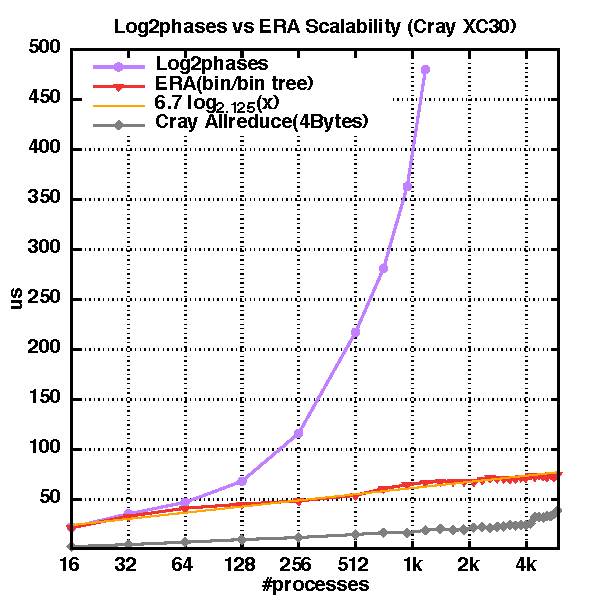
\includegraphics[height=.8\textheight]{eralog.pdf}

\end{frame}

\begin{frame}
  \frametitle{Post Failure Agreement Cost}

  \centering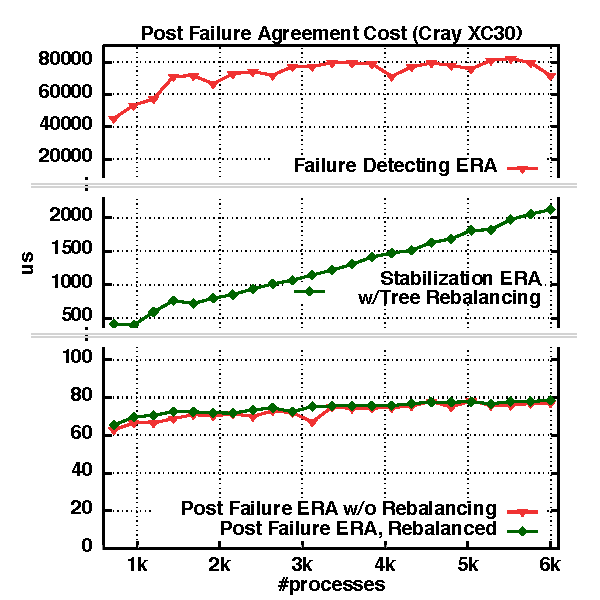
\includegraphics[height=.8\textheight]{eraaf.pdf}

\end{frame}

\begin{frame}
  \frametitle{FENIX \& S3D Performance}
  \begin{tabular}{p{.5\textwidth}p{.5\textwidth}}
    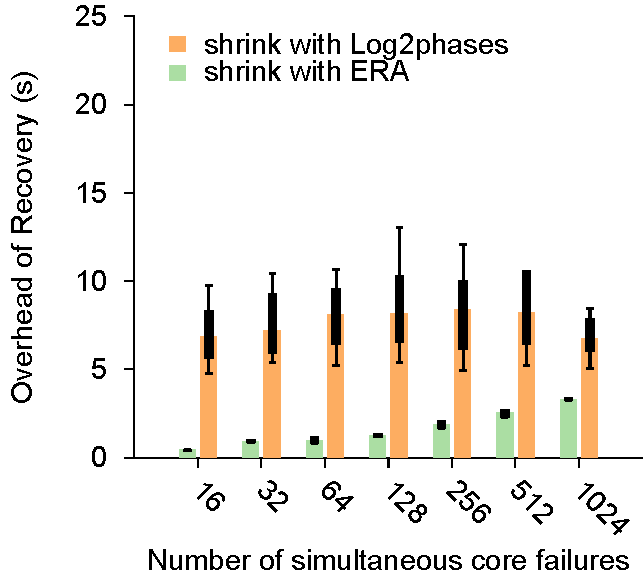
\includegraphics[width=\linewidth]{s3d_scalability_1.pdf}
    &
    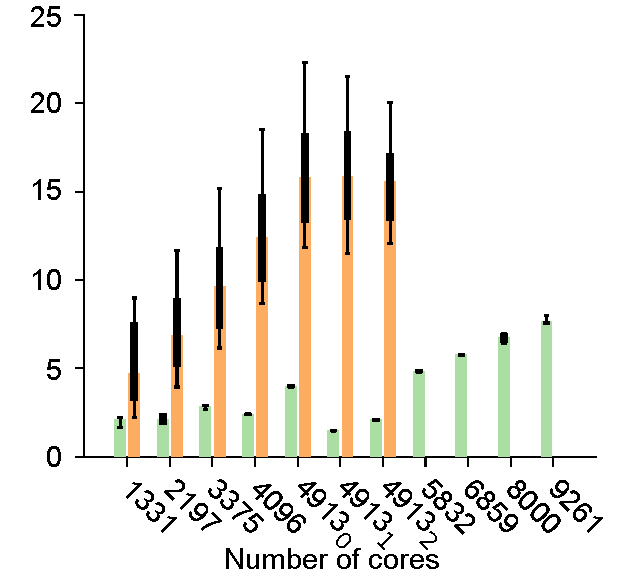
\includegraphics[width=\linewidth]{s3d_scalability_2_2.pdf}\\
    \centering Simultaneous failures on an increasing number of cores, over 2197
    total cores 
    &
     \centering 256-cores failure (\emph{i.e.}, 16 nodes) on an increasing number of
      total cores
  \end{tabular}
\end{frame}
